%\chapter*{Отчет}
\section*{Тренировочное задание}

Для выполнения тренировочного задания использовались настройки рабочей среды проекта, заданные в MS Project по умолчанию. Тип задачи по умолчанию: Фиксированный объем ресурсов.

Вариант 1 имеет следующие исходные данные (рис. \ref{p1}).
\begin{figure}[!h]
	\centering
	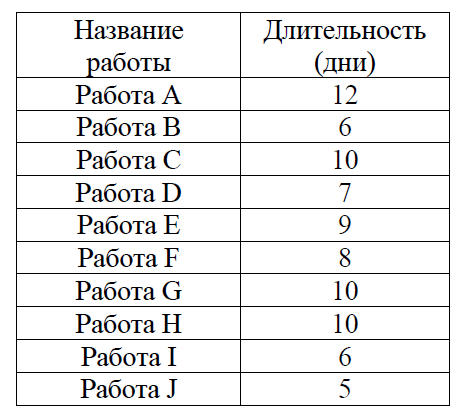
\includegraphics[width=0.5\linewidth]{inc/img/1.png}
	\caption{Исходные данные тренировочного задания}
	\label{p1}
\end{figure}

Дата начала проекта – 1-й рабочий день марта текущего года.

На рисунке \ref{p2} изображена полученная диаграмма Ганта.
\begin{figure}[!h]
	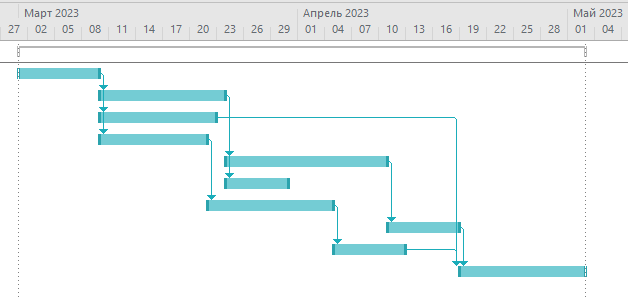
\includegraphics[width=1\linewidth]{inc/img/2.png}
	\caption{Диаграмма Ганта}
	\label{p2}
\end{figure}

\newpage
На рисунке \ref{p3} можно увидеть длительность проекта и дату завершения работ.
\begin{figure}[!h]
	\centering
	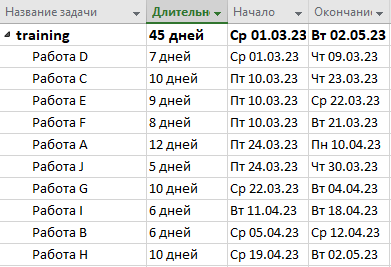
\includegraphics[width=0.7\linewidth]{inc/img/3.png}
	\caption{Длительность проекта и дата завершения работ}
	\label{p3}
\end{figure}

\section*{Лабораторная работа}
\textbf{Содержание проекта:} Команда разработчиков из \textbf{16 человек} занимается созданием карты города на основе собственного модуля отображения. Проект должен быть завершен в течение \textbf{6 месяцев}. Бюджет проекта: 50 000 рублей.

%\newpage
\subsection*{Задание №1: Настройка рабочей среды проекта}
Для выполнения задания №1 необходимо было установить дату начала проекта и настроить рабочую среду проекта (рис. \ref{p4.0}-\ref{p4}).

\begin{figure}[!h]
	\centering
	
\includegraphics[width=1\linewidth]{inc/img/4.0.png}
	\caption{Дата начала проекта}
	\label{p4.0}
\end{figure}

\newpage
\begin{figure}[!h]
	\centering
	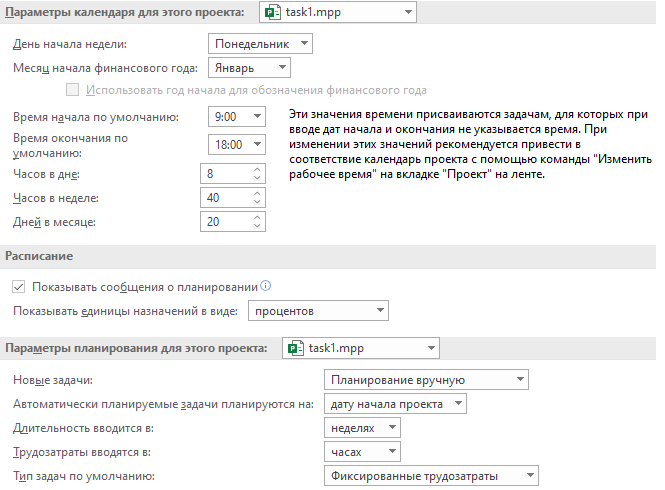
\includegraphics[width=1\linewidth]{inc/img/4.png}
	\caption{Настройка рабочей среды проекта}
	\label{p4}
\end{figure}

Кроме этого надо было отметить выходные и праздничные дни на ближайшие семь-восемь календарных месяцев от даты начала проекта, вывести на экран суммарную задачу проекта и заполнить вкладку \textit{Заметки} (рис. \ref{p5}-\ref{p5.0}).
\begin{figure}[!h]
	\centering
	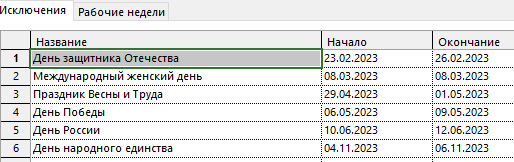
\includegraphics[width=1\linewidth]{inc/img/5.png}
	\caption{Выходные и праздничные дни}
	\label{p5}
\end{figure}

\begin{figure}[!h]
	\centering
	
\includegraphics[width=1\linewidth]{inc/img/5.0.png}
	\caption{Суммарная задача и Заметки}
	\label{p5.0}
\end{figure}

\newpage
\subsection*{Задание №2: Создание списка задач}
В задании №2 нужно было ввести список задач в соответствии с исходной таблицей. Результат представлен на рисунке \ref{p6}.
\begin{figure}[!h]
	\centering
	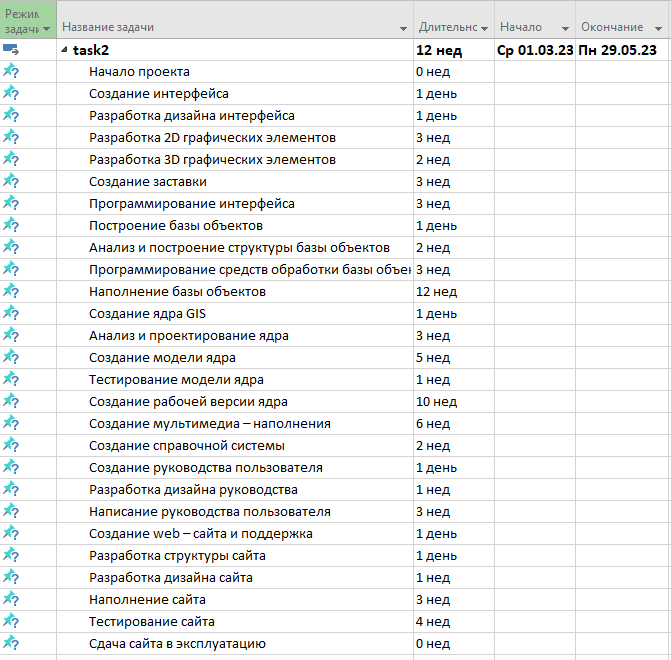
\includegraphics[width=1\linewidth]{inc/img/6.png}
	\caption{Cписок задач}
	\label{p6}
\end{figure}

\newpage
\subsection*{Задание №3: Структурирование списка задач}
В задании №3 нужно было провести группировку задач (рис. \ref{p7}).
\begin{figure}[!h]
	\centering
	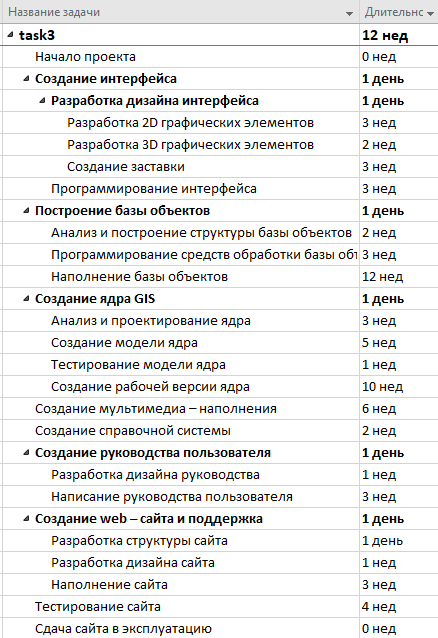
\includegraphics[width=0.7\linewidth]{inc/img/7.png}
	\caption{Группировка задач}
	\label{p7}
\end{figure}

\newpage
\subsection*{Задание №4: Установление связей между задачами}
В задании №4 нужно было установить связи между задачами. Результат представлен на рисунке \ref{p8}.
\begin{figure}[!h]
	\centering
	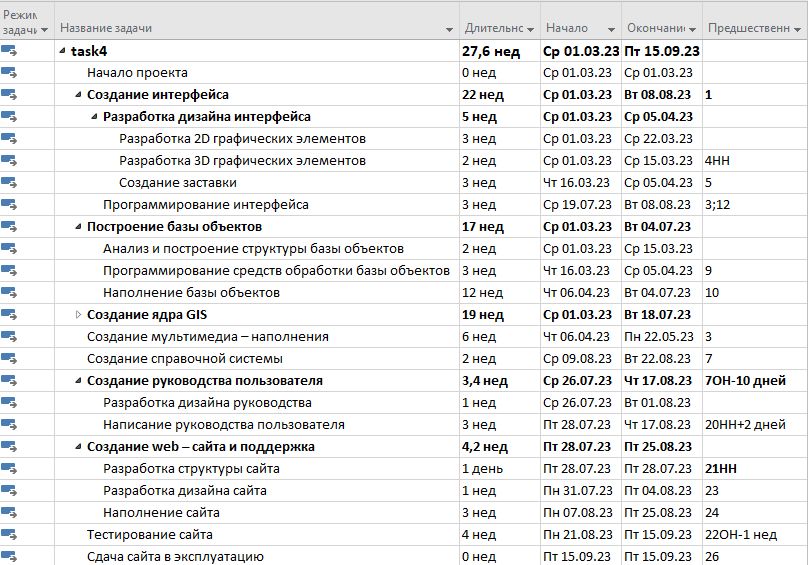
\includegraphics[width=1\linewidth]{inc/img/8.png}
	\caption{Задачи со связями}
	\label{p8}
\end{figure}

На рисунке \ref{p9} изображена полученная диаграмма Ганта.
\begin{figure}[!h]
	\centering
	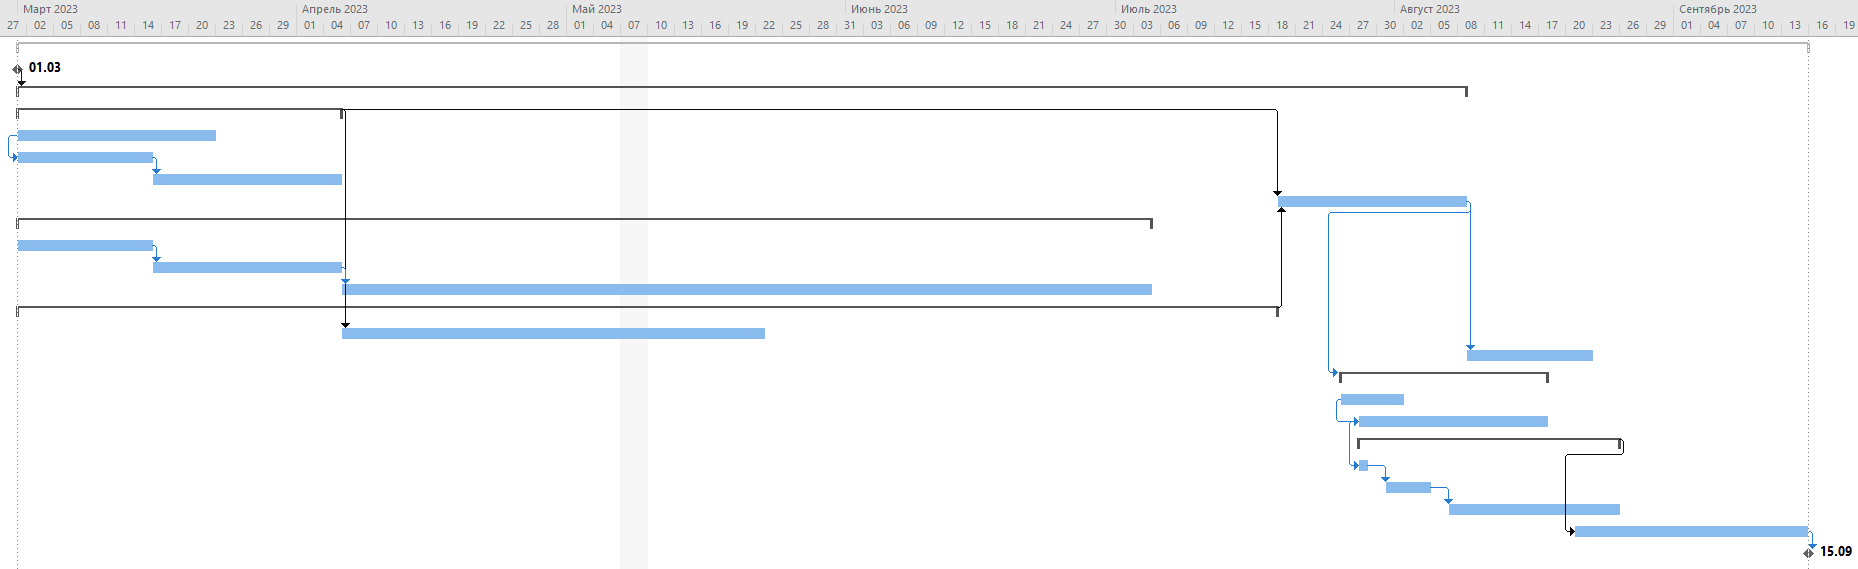
\includegraphics[width=1\linewidth]{inc/img/9.png}
	\caption{Полученная диаграмма Ганта}
	\label{p9}
\end{figure}

\section*{Выводы}
По итогу проделанной работы выяснилось что выполнение проекта не укладывается в отведенный срок 6 месяцев, а также были освоены возможности программы Microsoft Project для планирования проекта по разработке программного обеспечения.